%*****************************************
% Lab 06: PLA
%*****************************************
\chapter{Programmable Logic Array}\label{pla}

\section{Purpose}

This lab explores using a \ac{PLA} to simplify circuits that are designed for Boolean operations. A \ac{PLA} is an \ac{IC} that contains an array of \texttt{AND} and \texttt{OR} gates that can be linked in whatever way the circuit designer needs. A single \ac{PLA} can replace dozens of other gates and greatly simplify circuit design.

\section{Procedure}

\subsection{Equation One}

\begin{align}
	\label{eq:pla-01}
	(A'BC')+(AB'C')+(ABC)
\end{align}

In Lab \ref{bool} the circuit in Figure \ref{fig:pla-01} was developed to realize a Boolean expression.

\begin{figure}[H]
	\centering
	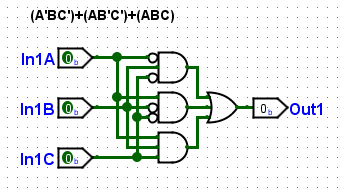
\includegraphics[width=\maxwidth{.95\linewidth}]{gfx/bool-04}
	\caption{Boolean Expression Realized}
	\label{fig:pla-01}
\end{figure}

This entire circuit can be realized in a single \ac{PLA} saving the cost of redundant \texttt{NOT/AND/OR} gates and improving the reaction time for the circuit while reducing the heat it generates.

The \LE \ac{PLA} component is a single box, as illustrated in \ref{fig:pla-02}. This \ac{PLA} has a 3-bit input attached, for inputs \textit{A}, \textit{B}, and \textit{C}, and a 1-bit output. The input is labeled \textit{ABC1} to indicate this is the input for equation one. 

\begin{figure}[H]
	\centering
	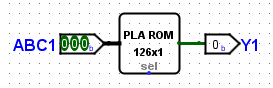
\includegraphics[width=\maxwidth{.95\linewidth}]{gfx/pla-01}
	\caption{Equation One}
	\label{fig:pla-02}
\end{figure}

Internally, a \ac{PLA} contains a matrix of \texttt{NOT/AND/OR} gates that are connected by the circuit designer. Figure \ref{fig:pla-03} illustrates the internal connections for the Equation One \ac{PLA}.

\begin{figure}[H]
	\centering
	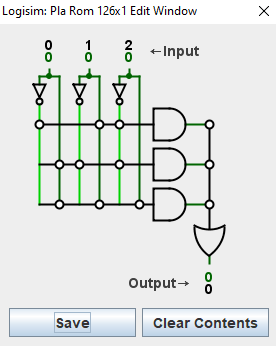
\includegraphics[width=\maxwidth{.95\linewidth}]{gfx/pla-02}
	\caption{PLA Internal Connections}
	\label{fig:pla-03}
\end{figure}

The three inputs are at the top of the \ac{PLA} and are labeled input 0, 1, and 2. Also, the values of those inputs is indicated immediately under the input number. At this time, all three are inputting a zero.

Notice that all three inputs are split and a \texttt{NOT} gate is inserted in one of the two split lines. By doing this, both \textit{A} and \textit{A'} are available on \ac{PLA} input zero. 

To the right of the grid is a column of three \texttt{AND} gates. These gates look a bit odd since there is only one input for each gate. This, though, simply represents that the \texttt{AND} gate has a variable number of inputs, depending on how the designer wired the circuit. For example, the top row has three connections to the top \texttt{AND} gate so it is a 3-input gate. The gate sizing happens automatically within the \ac{PLA} so the designer does not have to worry about it.

In the same way, there is a single \texttt{OR} gate near the bottom of the \ac{PLA}. While the diagram indicates that the \texttt{OR} gate has a single input, that gate actually has a variable input and will expand as necessary to support the circuit design. In this case, three separate rows are connected to the \texttt{OR} gate so it is a 3-input gate.

The very bottom of the \ac{PLA} is the output. It is numbered as output zero and its current value is zero.

To wire the \ac{PLA} device, the designer clicks on the wire intersections to place a connector (the small circle). Thus, row one of this device is connecting \textit{A'}, \textit{B}, and \textit{C'} to the top \texttt{AND} gate, which is then connected to the output \texttt{OR} gate.

Inspecting the connections for each row in this device should reveal that the top row is $ (A'BC') $, the second row is $ (AB'C') $ and the third row is $ (ABC) $, which are the three gates in the Boolean expression. The outputs from all three of those gates goes through an \texttt{OR} gate to the output. 

Thus, this one \ac{PLA} replaces all of the circuitry found in Figure \ref{fig:pla-01}.

Before moving on to the second equation, it will be helpful to take a look at the properties for a \ac{PLA}.

\begin{figure}[H]
	\centering
	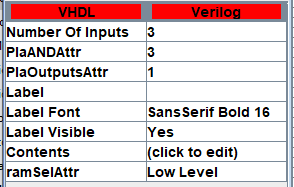
\includegraphics[width=\maxwidth{.95\linewidth}]{gfx/pla-03}
	\caption{PLA Properties}
	\label{fig:pla-04}
\end{figure}

The first property sets the number of inputs for the \ac{PLA}, the second property, \textit{PalANDAttr}, sets the number of \texttt{AND} gates and the third property, \textit{PlaOutputsAttr}, sets the number of outputs. These three properties ensure that the \ac{PLA} device can be used for many different applications. The three label properties are the same as found in most \LE components. Clicking the \textit{Contents} property will open the \ac{PLA} editor as illustrated in Figure \ref{fig:pla-03}\footnote{Important! The \LE \ac{PLA} seems to have a minor bug and the Contents editor will not always open. However, if the \textit{ramSelAttr} is clicked so its drop-down list is visible then the Contents \textit{(click to edit)} link will function properly. This is odd, but it will hopefully be corrected in a future iteration of \LE.}. Finally, the \textit{ramSelAttr} determines whether the \textit{Select} port, on the south edge of the \ac{PLA} is enabled on a high or low signal. The enable port is not used in this lab.

\subsection{Equation Two}

\begin{align}
	\label{eq:pla-02}
	(BCD')+(A'B'C)+(A'BCD')+(ABCD)
\end{align}

The subcircuit for Equation Two is very similar to that for Equation One, but the \ac{PLA} has different internal connections.

\begin{figure}[H]
	\centering
	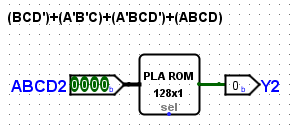
\includegraphics[width=\maxwidth{.95\linewidth}]{gfx/pla-04}
	\caption{Equation Two}
	\label{fig:pla-05}
\end{figure}

Notice that the input has four bits since the equation includes inputs \textit{A}, \textit{B}, \textit{C}, and \textit{D}. Also, the inputs and outputs include the number $ 2 $ to differentiate this subcircuit from the others.

When building this subcircuit be sure to use a \ac{PLA} device from the library instead of copy/paste from the subcircuit for Equation One. The internal connections for Equation Two are illustrated in Figure \ref{fig:pla-06}.

\begin{figure}[H]
	\centering
	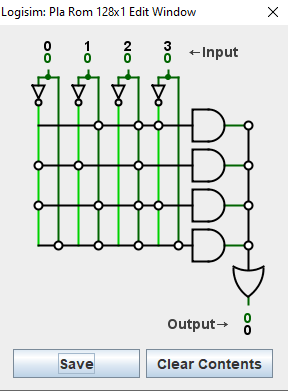
\includegraphics[width=\maxwidth{.95\linewidth}]{gfx/pla-05}
	\caption{Connections for Equation Two}
	\label{fig:pla-06}
\end{figure}

Notice that this equation includes two terms that have only three variables instead of four: (BCD') and (A'B'C). It does not cause a problem when a term in incomplete, only the variables present in the term are connected and the missing variable is ignored.

\subsection{Equation Three}

\begin{align}
	\label{eq:pla-03}
	&(A'BC')+(AB'C')+(ABC) \\
	\nonumber
	&(A'B'CD')+(A'BCD)+(AB'CD')+(ABCD')
\end{align}

The subcircuit for Equation Three is very similar to that for Equation Two, but the \ac{PLA} has different internal connections.

\begin{figure}[H]
	\centering
	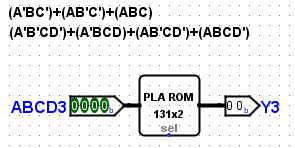
\includegraphics[width=\maxwidth{.95\linewidth}]{gfx/pla-06}
	\caption{Equation Three}
	\label{fig:pla-07}
\end{figure}

The major difference in Equation Three is that there are two outputs, so the \ac{PLA} must have two outputs specified and each equation is connected to the correct output.

\begin{figure}[H]
	\centering
	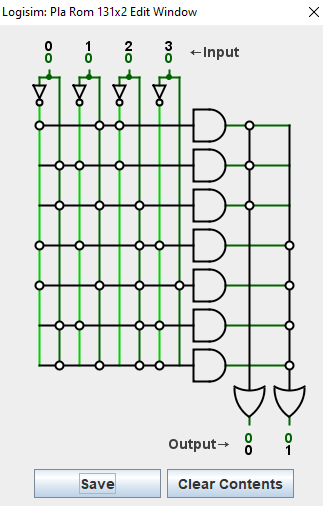
\includegraphics[width=\maxwidth{.95\linewidth}]{gfx/pla-07}
	\caption{Connections for Equation Three}
	\label{fig:pla-08}
\end{figure}

\section{Challenge}

On the \lstinline[columns=fixed]|main| circuit, wire a \ac{PLA} device using the same procedure that was used for circuits one, two, and three. That \ac{PLA} should display the correct outputs for equations \ref{eq:pla-04}.

\begin{align}
	\label{eq:pla-04}
	&(A'BC)+(ABC'D)+(A'B'CD) \\
	\nonumber
	&(BCD')+(A'B'C)+(A'BCD')+(ABCD)
\end{align}

The main circuit can be tested with the test vector provided with the lab starter circuit.

\section{Deliverable}

To receive a grade for this lab, complete the circuit. Be sure the standard identifying information is at the top left of the \lstinline[columns=fixed]|main| circuit, similar to: 

\bigskip
% The minipage environment keeps the three lines together - no page break.
\begin{minipage}{\linewidth}
	\begin{verbatim}
	George Self
	Lab 06: PLA
	September 17, 2019
	\end{verbatim}
\end{minipage}
\bigskip

Save the file with this name: \emph{\texttt{Lab06\_PLA}} and submit that file for grading.

